\documentclass[]{article}


\usepackage{float}
\usepackage[italian]{babel}

% Set page size and margins
% Replace `letterpaper' with`a4paper' for UK/EU standard size
\usepackage[letterpaper,top=3cm,bottom=3cm,left=3cm,right=3cm,marginparwidth=1.75cm]{geometry}

% Useful packages
\usepackage{amsmath}
\usepackage{graphicx}
\usepackage[colorlinks=true, allcolors=blue]{hyperref}


\title{SMSecure - Documentazione}
\author{Samuele Russo   matr.0512113317}


\begin{document}
\maketitle

\newpage

\tableofcontents

\newpage


\section{Introduzione}

    L'aumento esponenziale dell'utilizzo di dispositivi mobili ha reso gli SMS uno dei principali canali di comunicazione. Tuttavia, insieme a questa crescita, si è verificato un forte incremento del numero di spam SMS; ovvero messaggi caratterizzati da contenuti promozionali non richiesti, pubblicità ingannevoli o addirittura truffe; compromettendo l'efficienza e la sicurezza delle comunicazioni personali e professionali.


    \subsection{Obiettivi}

        Il mio progetto di FIA, prima esperienza personale in questo ambito, si propone di sviluppare un filtro anti-spam per migliorare l'esperienza degli utenti nel gestire i propri SMS. Ho deciso tale tematica perchè relativamente semplice, e di conseguenza in grado di farmi apprendere le basi del ML.

        Gli obiettivi principali includono:
        \begin{itemize}
            \item l'analisi approfondita di grandi quantità di SMS        estrapolati da un dataset.
            \item l'identificazione di feature associate ai               messaggi indesiderati.
            \item l'implementazione di un modello di apprendimento in grado di classificare in modo affidabile messagi spam e legittimi.
        \end{itemize}

    \subsection{Specifica PEAS}
        \begin{itemize}
            \item Performance (misure di prestazione adottate per valutare l’operato di un agente), nel mio caso verrà valutata la precisione di classificazione, ovvero il rapporto tra il numero di messaggi spam correttamente identificati e il totale dei messaggi classificati. Inoltre, sarà anche considerato il tasso di falsi positivi, ovvero messaggi legittimi che vengono erroneamente etichettati come spam.
            \item Environment (elementi che formano l’ambiente), nel mio caso sarà costituito dal flusso di messaggi ricevuti. 'vedi specifiche in 1.3'
            \item Actuators (attuatori disponibili all’agente per intraprendere le azioni), nel mio caso sarà la capacità del sistema di etichettare i messaggi in arrivo come spam o non spam.
            \item Sensors (sensori attraverso i quali l'agente riceve gli input percettivi), nel mio caso l'agente va ad acquisire i dati utili per classificare un messaggio, incluso il contenuto del messaggio, ma anche eventuali feature costruite (numero di parole ecc.)
        \end{itemize}

        \subsection{Caratteristiche dell'ambiente}
            L'ambiente è:
            \begin{itemize}
                \item Parzialmente osservabile, in quanto non si ha accesso alle informazioni del mittente.
                \item Stocastico, infatti i messaggi inviati dagli utenti sono influenzati da fattori non prevedibili.
                \item Singolo agente, in quanto c'è un solo questo filtro anti-spam in un client di messaggistica.
                \item Dinamico, difatti potrebbero venire a crearsi nuovi schemi di messaggi spam.
                \item Discreto, in quanto non sono presenti variabili continue (difatti una variabile continua potrebbe essere la frequenza di invio di un determinato mittente, ma io non ho trovato tale informazioni).
                \item Sequenziale, difatti il filtro anti-spam verrà pienamente influenzato dalle esperienze passate, per andare a prendere delle decisioni.
            \end{itemize}

        \newpage
        \subsection{Analisi del problema}
            Questo semplice progetto mira quindi a costruire un filtro anti-spam sms, si tratta quindi di un problema di Machine Learning, più nello specifico di un problema di apprendimento supervisionato, nonchè di classificazione. Nelle successive sezioni vado a descrivere tutte le problematiche che ho affrontato: dalla scelta dei dati, fino al deploy del modello.\\
            Per quanto riguarda le tecnologie che ho utilizzato per lo sviluppo del progetto, abbiamo:
            \begin{itemize}
                \item Python (in dettaglio le librerie per ML, come sickitLearn, Pandas,  ecc.),
                \item JupyterNotebook all'interno dell'IDE PyCharm
                \item GitHub per il versionamento
                \item Per quanto riguarda documentazione e presentazione overleaf (editor latex) e powerpoint rispettivamente.
            \end{itemize}
\newpage
\section{Data Understanding}
    Tale fase è composta da più punti:
    \begin{itemize}
        \item Acquisizione dei dati (scelta del dataset)
        \item Esplorazione dei dati
        \item Analisi della qualità dei dati
    \end{itemize}
    \subsection{Acquisizione dei dati}
        L'acquisizione dei dati è il processo di raccolta, ed organizzazione dei dati necessari per andare a creare un modello di ML. Con gli obiettivi chiari e definiti, sono andato alla ricerca di un dataset sul web, fino a trovarne uno molto interessante su Kaggle; una piattaforma, nonchè comunità online di data science. \\

        \begin{figure}[H]
            \centering
            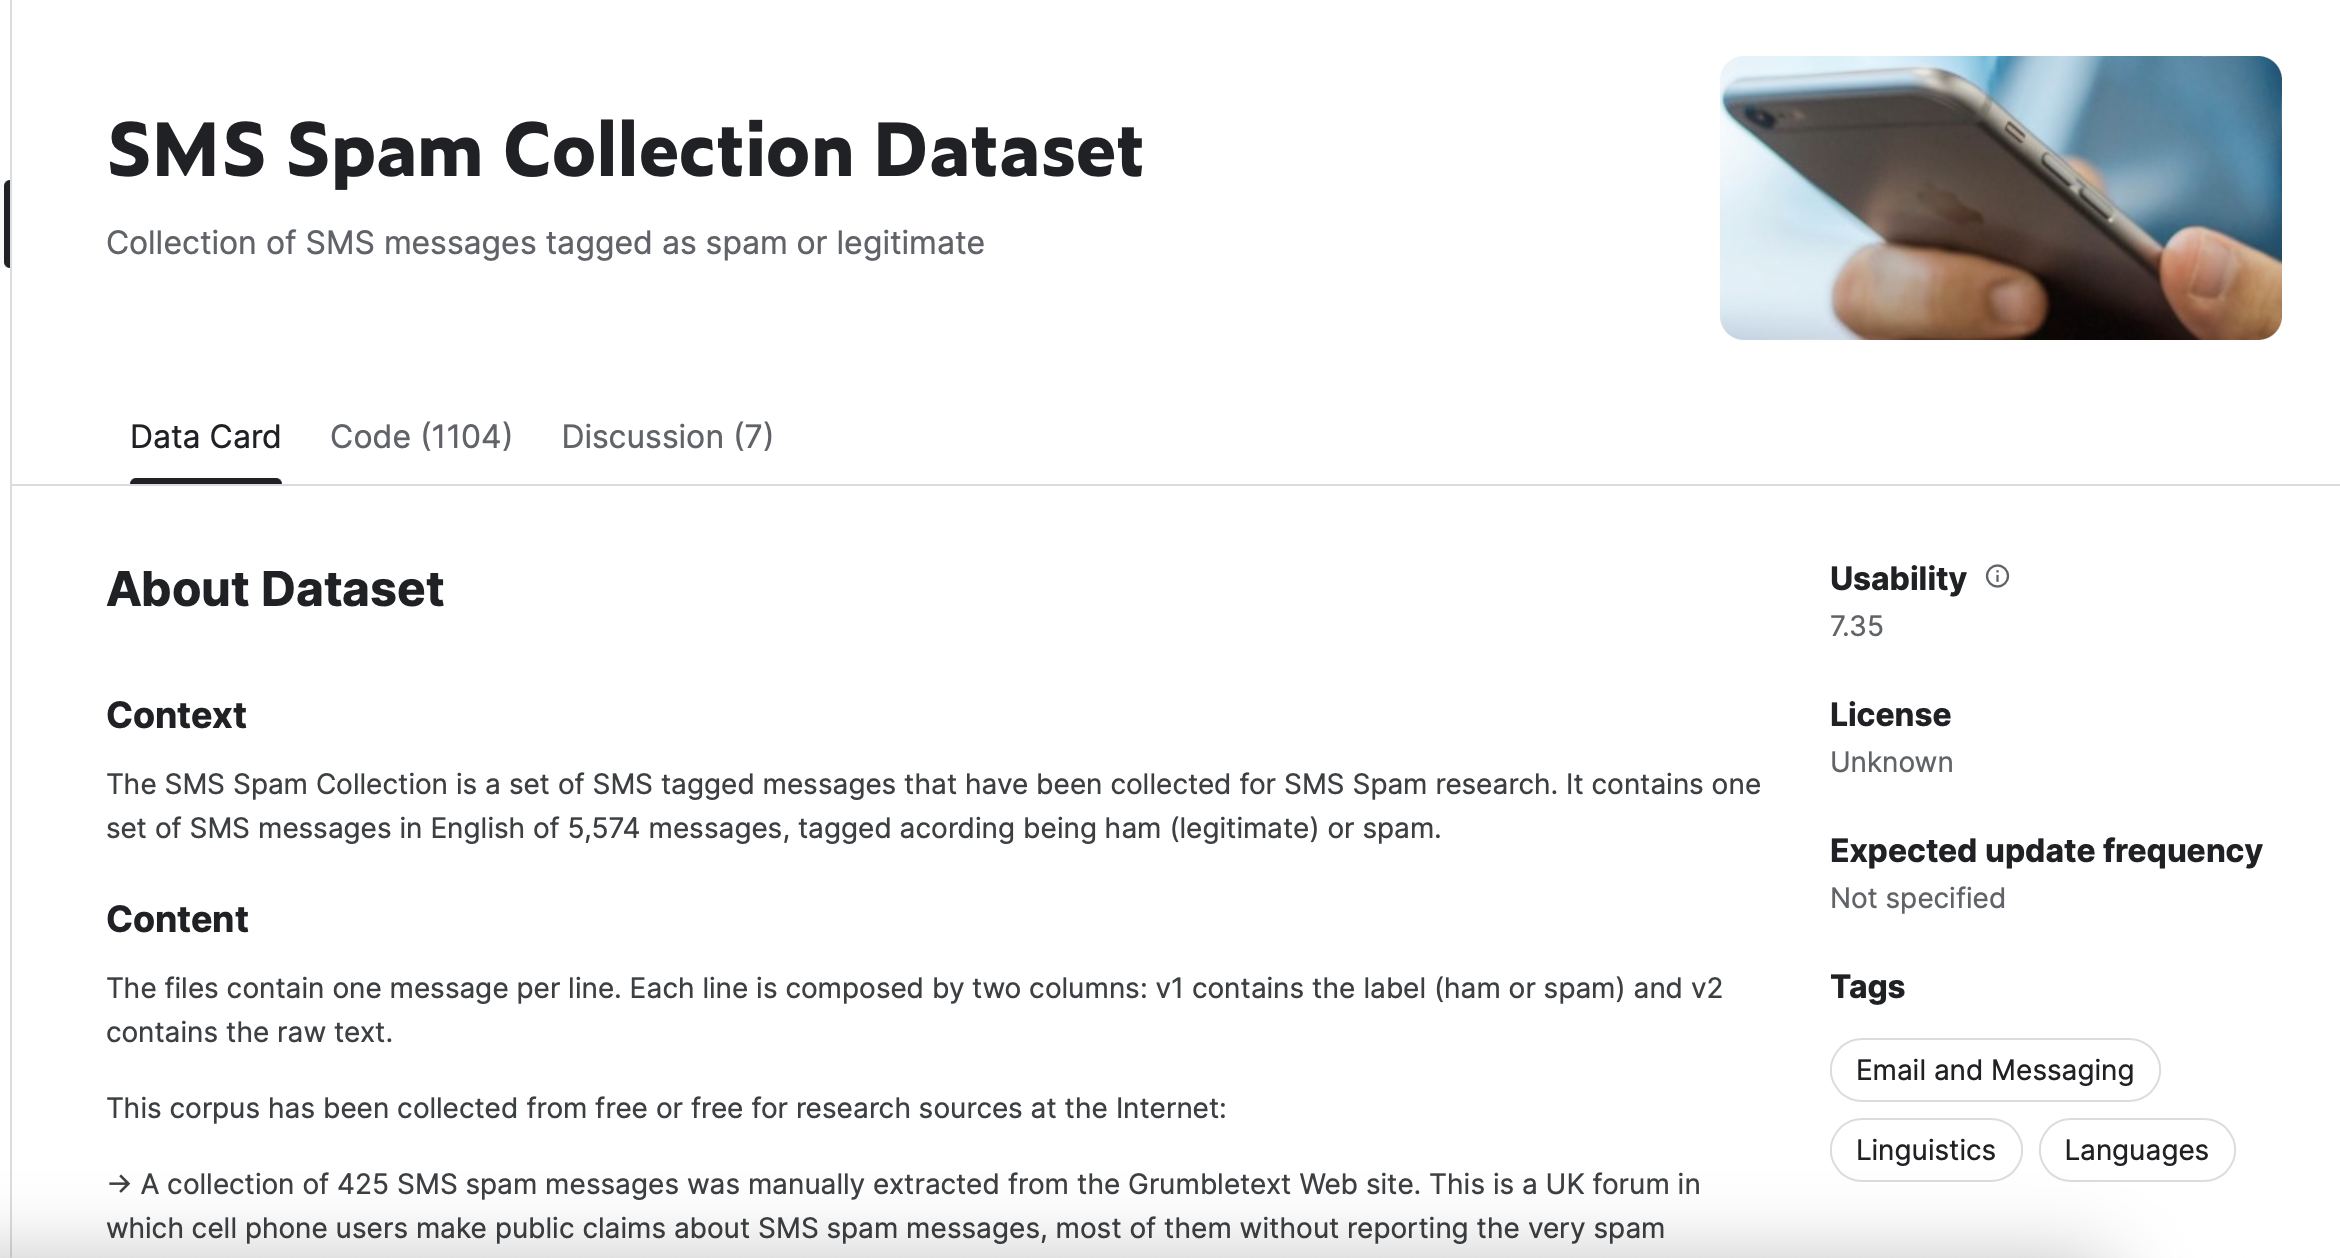
\includegraphics[width=1\linewidth]{images/kaggleDataset.png}
            \caption{Dataset su kaggle.com}
            \label{fig:enter-label}
        \end{figure}

    \subsection{Esplorazione dei dati}
        Il dataset in esame "SMS Spam Collection" è un insieme di messaggi SMS etichettati. Comprende 5.574 messaggi in inglese, suddivisi tra "ham" (legittimi) e "spam". Ogni messaggio è rappresentato da una riga con due colonne: una contiene l'etichetta (ham o spam) ed una contiene il testo grezzo dell'SMS. In questa fase vado ad analizzare, o meglio esplorare più nel dettaglio i dati per comprenderli e per scoprire informazioni rilevanti, tendenze, o relazioni. \\
        Quindi sono andato a fare una prima panoramica del dataset, andando a conteggiare quanti sample per ogni classe (ham/spam) fossero presenti, i nomi delle colonne, per poi passare alla vera esplorazione dei dati, volta quindi a trovare informazioni maggiormente rilevanti.\\
        Per un messaggio di testo è molto interessante andare ad osservare la sua lunghezza, il numero di parole al suo interno ed anche il numero di frasi. Non disponendo di tali feature sono andato a ricavarle, andando ad anticipare la \textbf{feature construction} della fase di Data Preparation.\\
        Per andare a ricavare queste feature dal testo ho utilizzato delle funzioni disponibili nella libreria nltk (conteggio parole e frasi), nonchè la funzione len() per calcolare il numero di caratteri. \\
        Per visualizzare eventuali trend e relazioni tra le varie feature, ho utilizzato alcuni grafici del libreria seaborn. Iniziamo ad analizzare i risultati ottenuti, partendo dal numero di caratteri.

        \begin{figure}[H]
            \centering
            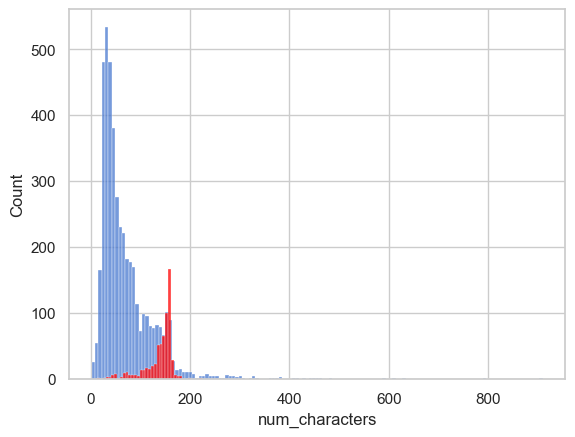
\includegraphics[width=0.6\linewidth]{images/num_char.png}
            \caption{numero di caratteri nei messaggi}
            \label{fig:enter-label}
        \end{figure}

        È da notare che in rosso sono rappresentati gli SMS spam, mentre in blu quelli ham. Sull'asse y la varibaile count indica il numero di volte in cui un determinato messaggio ha un certo numero di caratteri. Compreso ciò dal grafico è subito possibile notare che i messaggi spam hanno un numero di caratteri mediamente maggiore dei messaggi ham. \\
        Vediamo ora cosa emerge dal grafico che rappresenta il numero di parole.\\

        \begin{figure}[H]
            \centering
            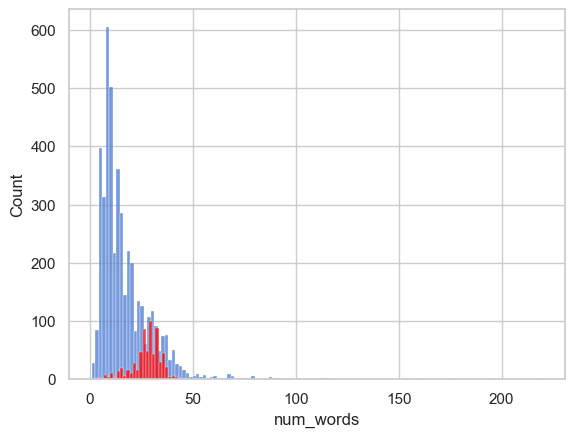
\includegraphics[width=0.6\linewidth]{images/num_words.png}
            \caption{numero di parole nei messaggi}
            \label{fig:enter-label}
        \end{figure}

        Si nota che vale lo stesso per il numero delle parole, difatti a rigor di logica il numero di parole è fortemente correlato al numero di caratteri, e quindi sarà lo stesso anche per il numero di frasi. Per vedere ancora più chiaramente tale correlazioni sono andato ad utilizzare un grafico riassuntivo, un pairplot.In tale tipo di grafico, ogni variabile numerica presente nel dataset viene confrontata con tutte le altre variabili numeriche tramite dei grafici a dispersione, che quindi consentono di visualizzare e individuare ancora meglio eventuali relazioni o tendenze.

        \begin{figure}[H]
            \centering
            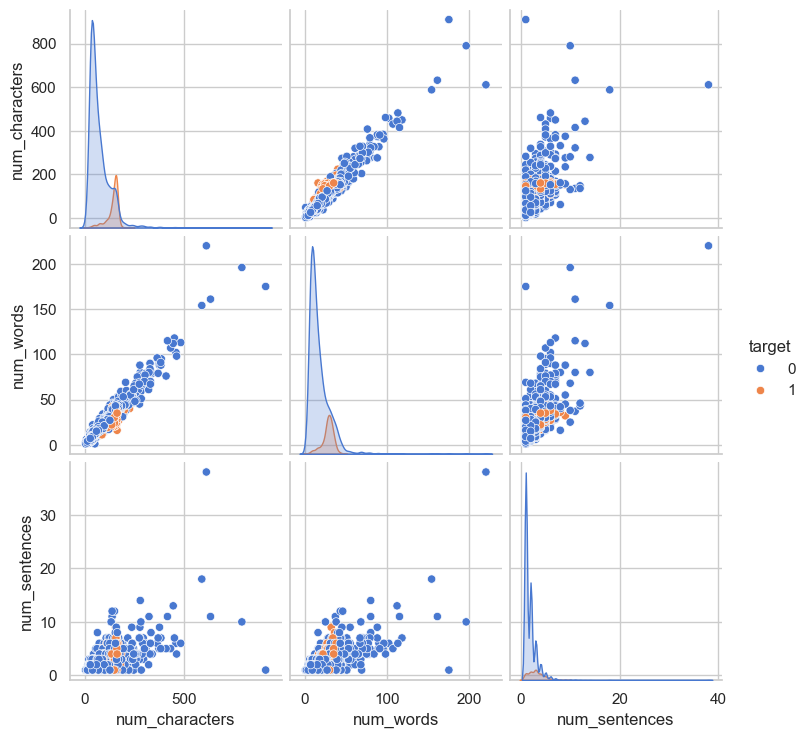
\includegraphics[width=1\linewidth]{images/sns_riassuntivo.png}
            \caption{pairplot riassuntivo}
            \label{fig:enter-label}
        \end{figure}

        Dal grafico emerge, ancora una volta, che:
        \begin{itemize}
        \item gli sms spam hanno in media un numero di caratteri maggiore
        \item gli sms spam hanno in media un numero di parole maggiore
        \item il numero di frasi è invece molto molto simile
        \end{itemize}

        Infine, per calcolare la correlazione tra le variabili, possiamo usare un'ulteriore strumento: la heatmap, una mappa che utilizza colori per visualizzare i valori dei coefficienti di correlazione tra le diverse coppie di variabili nel dataset, consentendo di individuare facilmente relazioni tra di esse. Le celle più scure o più chiare indicano correlazioni più forti o più deboli, rispettivamente. Le variabili sono fortemente correlate tra loro se hanno valori vicini a 1 o -1, mentre hanno una bassa correlazione se hanno valori vicini a 0.

        \begin{figure}[H]
            \centering
            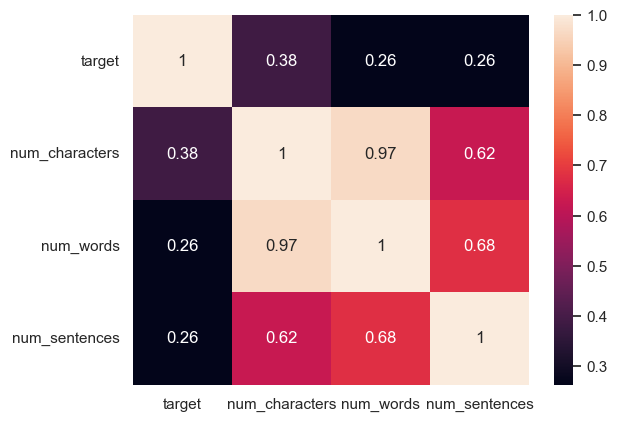
\includegraphics[width=0.7\linewidth]{images/matrice_corr.png}
            \caption{HeatMap}
            \label{fig:enter-label}
        \end{figure}

        E qui possiamo finalmente visualizzare l'effettiva correlazione tra le variabili. Si può notare con estrema facilità l'altissima correlazione tra il numero di caratteri e il numero di parole, cosa che è un pò meno marcata con il numero di frasi.\\
        Un'altra cosa davvero molto interessante è andare a visualizzare quali paroli sono più o meno frequenti nelle rispettive categoria di messaggi. Per fare ciò ho utilizzato la libreria wordCloud che permette di andare a generare una rappresentazione grafica semplice ed intuitiva. Ecco i due grafici realizzati:

        \begin{figure}[H]
            \centering
            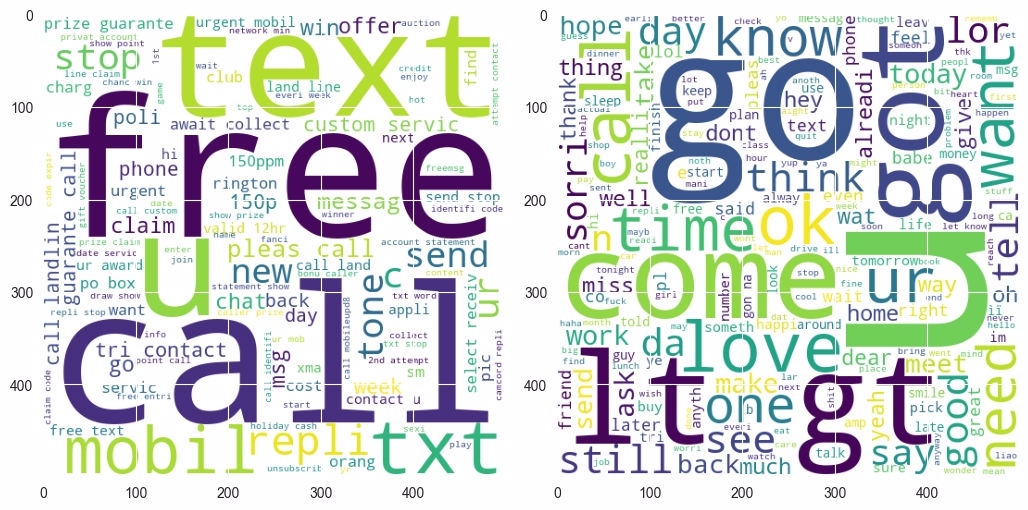
\includegraphics[width=0.7\linewidth]{images/wordCloudSpam.jpg}
            \caption{parole più frequenti (quelle di sinistra si riferiscono ai SPAM, quelle di destra agli HAM)}
            \label{fig:enter-label}
        \end{figure}

        Dai grafici emerge che le parole molto diffuse nei messaggi spam sono "free", "call", "text" e tantissime molte altre parole che difatti sono utilizzatissime nei messaggi spam, per  andare a fare pubblicità a servizi o tanto altro. Nel grafico di destra invece si possono osservare le parole più frequenti riscontrate nei messaggi ham, e come si può notare sono parole di utilizzo comune nei messaggi, ad esempio c'è anche la parola "ok".

    \subsection{Analisi della qualità dei dati}
        In questa fase vado ad analizzare i problemi di qualità dei dati rilevati durante la fase di esplorazione. A partire dai primi grafici usati nell'esplorazione si può notare che la quantità di messaggi ham, è molto maggiore rispetto alla quantità di messaggi spam.
        Difatti, andando ad approfondire, è risultata la presenza di:
        \begin{itemize}
            \item 4516 sms ham
            \item 653 sms spam
        \end{itemize}
        , graficamente:
        \begin{figure}[H]
            \centering
            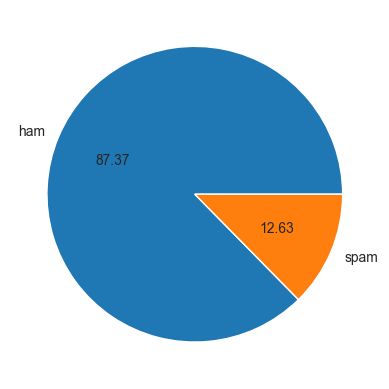
\includegraphics[width=0.5\linewidth]{images/sbilanciamento.png}
            \caption{percentuali di frequenza delle classi}
            \label{fig:enter-label}
        \end{figure}
        Questo indica un forte sbilanciamento dei dati, ed è quindi un problema che dovrà essere risolto. \\
        Altri problemi riscontrati:
        \begin{itemize}
            \item la presenza di 403 messaggi duplicati
            \item due colonne del dataset totalmente nulle
            \item nomi delle colonne non rappresentativi
        \end{itemize}
        Tali problemi saranno risolti nella sezione successiva, ovvero nella \textbf{Data Preparation}.

    \newpage
    \section{Data Preparation}
        Tale fase mira a rendere i dati adatti per l'utilizzo nelle fasi successive del processo. Questo processo include più punti:
        \begin{itemize}
            \item data cleaning
            \item feature scaling
            \item feature selection
            \item data balancing
        \end{itemize}
         Quindi l'output di questa fase sarà un insieme di dati di input, che saranno utilizzati durante la modellazione dell'algoritmo di ML.
    \subsection{Data Cleaning}
        In questa fase sostanzialmente vanno corretti alcuni dei problemi individuati in fase di Data understanding: valori nulli e duplicati; per poi passare alla trasformazione dei dati in modo da poter essere utilizzati e "dati in pasto" ad un algortimo di ML.\\
        Quindi, innanzitutto, ho eliminato completamente due colonne dal dataset poiché erano completamente vuote. Successivamente, ho rimosso 403 valori duplicati. Inoltre, ho rinominato le colonne come "target" e "text" in quanto i nomi precedenti ("v1", "v2") erano ambigui e poco rappresentativi. Successivamente, ho proceduto sostituendo le variabili target "spam" e "ham" rispettivamente con 1 e 0. Ho adottato questa procedura per garantire la compatibilità con gli algoritmi di classificazione binaria.

        Avendo a che fare con del testo, il "mining", ovvero l'estrazione di semantica dai testi è leggermente complicata e va adattata al contesto. I maggiori problemi da affrontare riguardano il fatto che nel linguaggio naturale son presenti più modi per esprimere stessi concetti, possono esserci errori grammaticali; o più in generale l'estrazione delle informazioni viene difficile. Nel mio caso trattandosi di testo di SMS, ho deciso di attuare le seguenti trasformazioni:
        \begin{itemize}
            \item Tokenizzato in parole
            \item Portato tutto le parole in minuscolo
            \item Rimosso i caratteri non alfanumerici
            \item Rimosso le stopwords
            \item Stemming delle parole
        \end{itemize}
        Tutti queste trasformazioni da effettuare hanno scopi ben precisi; infatti la \textbf{tokenizzazione} aiuta a trattare le parole individualmente durante l'analisi;
        \textbf{portare tutto in minuscolo} aiuta ad eliminare la distinzione tra maiuscole e minuscole, garantendo coerenza nell'analisi; la \textbf{rimozione caratteri non alfanumerici}va ad eliminare simboli e punteggiatura concentrando l'attenzione sulle informazioni sostanziali delle parole; la \textbf{rimozione delle stopwords}che sono parole comuni che spesso non contribuiscono significativamente al significato aiuta a ridurre il rumore nei dati; ed infine lo \textbf{stemming} che riduce le parole alle loro radici (stems) fa in modo che parole simili siano rappresentate in modo uniforme, semplificando l'analisi.
        Ho realizzato ciò usando funzioni e dizionari preesistenti, andando solamente ad accorpare il tutto in un'unica funzione.
        \newpage
        \begin{verbatim}

            def transform_text(text):
                text = text.lower() #tutto in minuscolo
                text = nltk.word_tokenize(text) #tokenizzazione

                #Rimozione caratteri non alfanumerici
                y = []
                for i in text:
                    if i.isalnum():
                        y.append(i)

                text = y[:]
                y.clear()

                # Rimozione stopwords
                for i in text:
                    if i not in stopwords.words('english') and i not in string.punctuation:
                        y.append(i)

                text = y[:]
                y.clear()

                #stemming (ps è l'oggetto portStemmer)
                for i in text:
                    y.append(ps.stem(i))

                #Restituisce il testo pre-elaborato come una stringa di parole separate tra spazi.
                return " ".join(y)

        \end{verbatim}
        Quindi dopo aver definito tale funzione, ho semplicemente processato tutto il testo degli SMS per poi inserirlo in una nuova colonna del dataset.

    \subsection{Feature Scaling}
        In questa fase si vanno ad utilizzare delle tecniche per normalizzare o scalare i valori delle caratteristiche in modo da avere una scala uniforme. Questo serve per evitare che caratteristiche con scale molto diverse influenzino negativamente gli algoritmi di apprendimento. Nel mio caso ho notato che le scale fra il numero di caratteri, numero di parole e numero di frasi sono molto differenti; difatti i caratteri arrivano anche a oltre 180, il numero di parole non supera nella maggiorparte dei casi 50, ed infine il numero frasi non supera le 10. Quindi ho ritenuto opportuno andare a normalizzare tali valori, e per farlo ho usato una funzione della libreria sklearn.
        \begin{verbatim}
            #colonne che voglio normalizzare
            features_to_normalize = ['num_characters', 'num_words', 'num_sentences']

            #oggetto che permette la normalizzazione
            scaler = MinMaxScaler()

            df[features_to_normalize] = scaler.fit_transform(df[features_to_normalize])
        \end{verbatim}

        \subsection{Feature Selection}
            La feature selection è il processo in cui si va a scegliere un sottoinsieme delle caratteristiche più rilevanti dai dati originali per andare a ridurre la complessità del modello e si conseguenza migliorare le prestazioni. Per far ciò si utilizza anche il Feature Engineering ovvero il processo nel quale il progettista utilizza la propria conoscenza del dominio per determinare le feature e dare più o meno enfasi ad esse. Nel mio caso, osservando i valori dopo, o comunque prima della fase di Feature Scaling, ho notato che: il numero di frasi dei messaggi è una feature a bassa varianza (i suoi valori variano poco) quindi con questa è una feature non rilevante per la classificazione; di conseguenza ho deciso di eliminarla per ridurre la complessità generale. In questa fase si vanno anche ad effettuare altre operazioni, come ad esempio la feature construction, in cui il progettista va a costruire nuovi feature a partire dai dati. Io già in precedenza ho costruito, partendo dal testo, il numero di frasi, di parole e di caratteri per ogni messaggio.

        \subsection{Data Balancing}
            Il Data Balancing sono un insieme di tecniche per andare a convertire un dataset sbilanciato, ovvero con una distribuzione sbilanciata delle classi nei dati, in un dataset bilanciato. Difatti avere un dataset sbilanciato può portare a diversi problemi, tra questi previsioni sbilanciate e innaccurate, nonchè overfitting.
            Le tecniche applicabili sono due:
            \begin{itemize}
                \item Undersampling
                \item Oversampling
            \end{itemize}
            con la presenza di varianti che includono il clustering, per evitare alcuni inconvenienti, come ad esempio andare ad eliminare righe molto utili per l'apprendimento. In generale, in base alla propria situazione sarà, piò o meno adatta una precisa tecnica.
            Nel mio caso, il dataset è fortemente sbilanciato, con una presenza maggiore di istanze della classe ham. Quindi le possibilità erano due:
            \begin{itemize}
                \item Eliminare istanze della classe ham
                \item Aumentare le istanze della classe spam
            \end{itemize}
            Tra le due, per evitare duplicazione di entry e quindi overfitting, ho deciso di optare per la prima opzione, andando però a considerare l'uso dell' \textbf{undersampling con clustering}, per evitare di eliminare istanze rilevanti per l'apprendimento.













%\bibliographystyle{alpha}%
%\bibliography{sample}%

\end{document}